% OGP: A BGP-Inspired Federation Protocol for Human-Mediated AI Gateway Interoperability
% HotNets 2026 Submission
% Author: David Proctor
%
% Compile with:
%   pdflatex hotnets2026.tex
%   bibtex hotnets2026
%   pdflatex hotnets2026.tex
%   pdflatex hotnets2026.tex
%
% Requires: ACM sigconf class (acmart.cls)
% Download: https://www.acm.org/publications/proceedings-template

\documentclass[sigconf,nonacm]{acmart}

\usepackage{listings}
\usepackage{booktabs}
\usepackage{graphicx}
\usepackage{xcolor}
\usepackage{tikz}
\usetikzlibrary{arrows.meta, positioning, shapes.geometric}

\lstset{
  basicstyle=\small\ttfamily,
  breaklines=true,
  frame=single,
  columns=fullflexible,
}

% Minimal JSON language definition for listings (not built-in)
\lstdefinelanguage{json}{
  basicstyle=\small\ttfamily,
  showstringspaces=false,
  breaklines=true,
  literate=
   *{0}{{{\color{blue}0}}}{1}
    {1}{{{\color{blue}1}}}{1}
    {2}{{{\color{blue}2}}}{1}
    {3}{{{\color{blue}3}}}{1}
    {4}{{{\color{blue}4}}}{1}
    {5}{{{\color{blue}5}}}{1}
    {6}{{{\color{blue}6}}}{1}
    {7}{{{\color{blue}7}}}{1}
    {8}{{{\color{blue}8}}}{1}
    {9}{{{\color{blue}9}}}{1}
    {:}{{{\color{black}{:}}}}{1}
    {,}{{{\color{black}{,}}}}{1}
    {\{}{{{\color{black}{\{}}}}{1}
    {\}}{{{\color{black}{\}}}}}{1}
    {[}{{{\color{black}{[}}}}{1}
    {]}{{{\color{black}{]}}}}{1},
}

% HotNets: 6-page limit, no abstract word limit specified
\settopmatter{printacmref=false}
\renewcommand\footnotetextcopyrightpermission[1]{}
\pagestyle{plain}

\begin{document}

\title{OGP: A BGP-Inspired Federation Protocol for Human-Mediated AI Gateway Interoperability}

\author{David Proctor}
\affiliation{%
  \institution{Trilogy AI Center of Excellence}
  \country{USA}
}
\email{david.ai@trilogy.com}

\begin{abstract}
AI assistants are proliferating but remain organizationally siloed.
When users from different organizations need their agents to collaborate---on
legal review, insurance authorization, or shared project coordination---no
protocol exists for establishing the required cross-boundary trust.
Existing protocols address adjacent problems: MCP attaches tools to single
agents, A2A delegates tasks within organizational boundaries, and ANP
discovers agents on the open web.
None address the fundamental challenge of two humans granting their AI
systems permission to work together directly, under explicit scoped
authorization, with unilateral revocability.

We present the Open Gateway Protocol (OGP), a federation protocol that
borrows its trust and policy model from BGP (Border Gateway Protocol).
OGP treats each AI gateway as an autonomous system and establishes
bilateral peer relationships through human-approved handshakes, per-peer
scope negotiation, and Ed25519 per-message authentication.
A three-layer Doorman enforces scope at runtime.
An OSPF-inspired state machine tracks federation health over time.
We describe the protocol design, analyze its security properties against
a published threat taxonomy, and present microbenchmark results showing
that the cryptographic and enforcement overhead is sub-millisecond at
every layer, adding negligible latency to agent-to-agent communication.
OGP is implemented as an open-source reference daemon (\texttt{@dp-pcs/ogp},
v0.11.3) with nearly 400 commits over three months and multiple active
cross-organizational deployments.
\end{abstract}

\maketitle

%%------------------------------------------------------------------
\section{Introduction}
%%------------------------------------------------------------------

The past year has produced a proliferation of AI agent protocols.
MCP~\cite{mcp2024} standardizes how agents attach to tools.
A2A~\cite{a2a2025} standardizes how agents delegate tasks to one another.
ANP~\cite{anp2024} proposes a decentralized open web for agent discovery.
Yet none of these protocols address a problem that arises the moment two
people try to use their AI assistants together: \emph{how do two gateways
owned by different humans establish trust?}

Consider two concrete scenarios:

\vspace{0.3em}
\noindent\textbf{Legal review.} Alice's firm is reviewing a contract with
Bob's firm. Alice's AI assistant has context on her firm's position; Bob's
has context on his. Neither party wants to share raw context with the
other---they want their agents to exchange structured, scoped, attributable
information without either firm's data crossing an uncontrolled boundary.

\vspace{0.3em}
\noindent\textbf{Project coordination.} David's agent and Cosmo's agent are
collaborating on a cross-organizational software project. They need to
exchange status updates, query each other's project decisions, and push
signed contributions to a shared record---but David does not want Cosmo's
agent to access his calendar, his email context, or any capability he has
not explicitly granted.

\vspace{0.3em}

No existing protocol addresses these scenarios.
MCP runs within a single trust boundary.
A2A assumes a shared organizational identity provider and targets
intra-organizational orchestration~\cite{survey2025}.
ANP provides identity and discovery for the open public web but has no
bilateral approval mechanism---any authenticated agent can connect to any
other~\cite{anp2024}.
ActivityPub~\cite{activitypub2018} federates social content, not agentic tasks.

We present \textbf{Open Gateway Protocol (OGP)}, which fills this gap by
treating AI gateway federation the same way BGP treats autonomous network
federation: bilateral human approval, explicit per-peer policy, and
cryptographic authentication on every message.

OGP makes four contributions:
\begin{enumerate}
\item A \textbf{gateway-level federation protocol} with a human-mandatory
  approval handshake, cleanly separating the trust decision (human-made,
  once) from message exchange (agent-automated, many times).
\item A \textbf{three-layer scope model} (capability advertisement,
  per-peer negotiation, runtime enforcement) that separates what a gateway
  supports from what a specific peer is granted.
\item An \textbf{OSPF-inspired federation lifecycle state machine} that
  tracks peer health and enables graceful degradation and tombstoning.
\item A \textbf{reference implementation} (open source, nearly 400 commits,
  npm package \texttt{@dp-pcs/ogp}) deployed across multiple independent,
  geographically distributed organizational gateways, with microbenchmarks
  demonstrating sub-millisecond enforcement overhead at every layer.
\end{enumerate}

%%------------------------------------------------------------------
\section{Problem Statement}
%%------------------------------------------------------------------

\subsection{The Cross-Boundary Trust Gap}

Existing agent protocols can be placed on two axes: the trust model
they assume (service-level vs.\ human-level), and the scope they control
(single-agent vs.\ cross-org). Table~\ref{tab:protocols} shows the landscape.

\begin{table}[h]
\centering
\caption{Positioning of AI agent protocols by trust model and scope.}
\label{tab:protocols}
\small
\begin{tabular}{lllll}
\toprule
Protocol & Trust model & Scope & Human approval & Signing \\
\midrule
MCP      & Host-delegated & Tool/agent & Guideline only & None \\
A2A      & OAuth + cards  & Intra-org  & Not required   & JWS \\
ANP      & DID crypto     & Open web   & High-risk only & ECDHE \\
ACP      & DID + VC       & Multi-org  & Not required   & VC \\
ActivityPub & Impl.-delegated & Social & Optional & Advisory \\
\textbf{OGP} & \textbf{Bilateral} & \textbf{Cross-org} & \textbf{Mandatory} & \textbf{Ed25519} \\
\bottomrule
\end{tabular}
\end{table}

The gap is specific: no protocol makes human approval of federation
\emph{mandatory at the protocol level}, enforces \emph{per-peer scoped
permissions} on every message, and provides \emph{unilateral revocability}
with cryptographic tombstoning to prevent silent re-trust.

\subsection{Why Existing Approaches Fail}

\textbf{Shared identity providers} (OAuth, enterprise SSO) require both
parties to be enrolled in the same identity system---which is precisely
what fails in cross-organizational scenarios between parties with no
pre-existing relationship.

\textbf{API key exchange} provides authentication but no scope model:
the API key either works or it does not. There is no per-intent
granularity, no topic restrictions, no sliding-window rate limiting,
and no revocation semantics beyond deleting the key out-of-band.

\textbf{Trust-on-first-use} (ActivityPub Follow, ANP connection)
makes the approval optional or automated. This is appropriate for
social networks; it is inappropriate for sensitive cross-organizational
AI collaboration where the human must remain the arbiter of what their
agent is authorized to do on their behalf.

%%------------------------------------------------------------------
\section{Related Work}
%%------------------------------------------------------------------

\textbf{MCP}~\cite{mcp2024} (Anthropic, 2024) is a JSON-RPC protocol
for attaching tools and resources to a single LLM agent.
Trust is entirely delegated to the host application; the spec explicitly
states ``MCP itself cannot enforce these security principles at the
protocol level.'' MCP has no message signing, no peer-to-peer federation
concept, and no revocation mechanism.

\textbf{A2A}~\cite{a2a2025} (Google, 2025--2026) enables task delegation
between agents via Agent Cards published at \texttt{/.well-known/agent.json}.
Identity is Agent-Card + OAuth. A2A does not mandate human approval
for new agent relationships and targets intra-organizational enterprise
orchestration. Its scope control relies on OAuth scopes; a recent
security analysis identified ``insufficiently granular token scope'' as
a known risk~\cite{security2026}. A2A and OGP are complementary:
OGP establishes cross-org gateway trust; A2A can be used internally
to delegate tasks within a trusted boundary.

\textbf{ANP}~\cite{anp2024} (2025, open-source) proposes W3C DIDs
(\texttt{did:wba}) for decentralized agent identity and JSON-LD for
semantic capability discovery. ANP is designed for the open public web
and prioritizes discovery over bilateral approval. It explicitly flags
revocation infrastructure (CRLs, status protocols) as an open problem.
The trust model assumes ``least trust'' but has no mandatory human
approval gate for federation.

\textbf{ACP.} The name ``ACP'' refers to two distinct efforts. The
IBM/BeeAI Agent Communication Protocol (now hosted by the Linux Foundation)
defines a RESTful, MIME-typed messaging protocol with session management
and optional DID-based identity~\cite{survey2025}. Separately, a recent
academic proposal of the same name~\cite{acp2026} describes a federated
orchestration model built on decentralized identity and verifiable
credentials, in which orchestration is an emergent property with no central
master agent. The latter is closest to OGP in security posture---decentralized
identity with no central trust root---but, like the others, it establishes
trust through verifiable credentials rather than a mandatory human approval
gate, and does not provide unilateral revocation with anti-re-trust semantics.

\textbf{ActivityPub}~\cite{activitypub2018} (W3C, 2018) federates
social content between independently operated servers.
Its trust model is implementation-delegated; the spec notes ``there
are no strongly agreed upon mechanisms for authentication'' at
standardization time. Message signing is advisory, not mandatory.

\textbf{BGP}~\cite{rfc4271} provides the conceptual model for OGP's
peering architecture. The peering handshake, bilateral policy
negotiation, and peer lifecycle state machine in OGP are all derived
from BGP's design. OGP does not implement route computation, path
selection, or multi-hop forwarding---it takes only the peering model.
Notably, BGP-4 has no native message authentication, and its trust
failures (e.g., route hijacks) motivated later retrofits such as RPKI and
BGPsec. OGP adopts BGP's peering and policy model while authenticating
every message from the outset, avoiding that original sin.

\textbf{Trust Fabric}~\cite{trustfabric2025} (2025) proposes a decentralized
interoperability and economic-coordination layer for the ``agentic web,''
combining DID-based discovery, verifiable-credential agent cards, and a
behavioral-attestation trust layer. It targets open-web, marketplace-scale
agent interaction; OGP instead targets closed, bilateral, human-approved
relationships between two specific organizations.

A recent security threat taxonomy~\cite{security2026} analyzed MCP, A2A,
Agora, and ANP and identified \emph{twelve protocol-level risks} across three
categories---authentication and access control, supply-chain and ecosystem
integrity, and operational integrity and reliability---scored over a
creation/operation/update lifecycle. OGP's design structurally addresses the
entire authentication-and-access-control category and selected risks in the
other two (Table~\ref{tab:threats}); the remainder are agent- or runtime-layer
concerns outside the gateway boundary.

\begin{table}[h]
\centering
\caption{Protocol-level risks from the taxonomy of~\cite{security2026} that
OGP structurally mitigates, grouped by the taxonomy's three categories.
Risks at the agent/runtime layer (e.g., sandbox escape, tool poisoning, code
injection, rug pulls) are out of OGP's scope.}
\label{tab:threats}
\small
\begin{tabular}{p{0.40\columnwidth}p{0.50\columnwidth}}
\toprule
Risk & OGP mitigation \\
\midrule
\multicolumn{2}{l}{\textit{Authentication \& access control}} \\
Lack of authentication & Ed25519 verify on every message \\
Weak/limited access control & Three-layer Doorman per-peer grant \\
Naming collision \& impersonation & Public key \emph{is} the identity \\
No token-lifetime limit & 5-min freshness window + nonce; no bearer token \\
Insufficiently granular scope & Per-intent, per-topic grant + rate limit \\
\midrule
\multicolumn{2}{l}{\textit{Supply chain \& ecosystem integrity}} \\
Installer spoofing & OGP Apps: publisher key checked vs.\ trusted peer record + consent gate \\
\midrule
\multicolumn{2}{l}{\textit{Operational integrity \& reliability}} \\
Post-update privilege persistence & Tombstoning; grant re-read per request; no silent re-trust \\
Configuration drift & Stored grant is the single source of truth, re-evaluated per request \\
\bottomrule
\end{tabular}
\end{table}

%%------------------------------------------------------------------
\section{Protocol Design}
%%------------------------------------------------------------------

\subsection{Identity and Discovery}

Each OGP gateway generates an Ed25519 keypair on first start.
The \emph{public key is the identity}: there is no separate identifier
that must be resolved against an external registry.
On macOS, the private key is stored in an instance-specific Keychain entry;
on other platforms it is encrypted at rest using an operator-provided secret.

Gateways publish a signed discovery card at \texttt{GET /.well-known/ogp}:

\begin{lstlisting}[language=json, caption={Discovery card (abbreviated).}]
{
  "publicKey": "302a300506032b65...",
  "displayName": "David Proctor / Junior",
  "gatewayUrl": "https://ogp.david.example.com",
  "capabilities": {
    "intents": ["message","agent-comms",
      "project.contribute","project.query"],
    "features": ["relay","rendezvous"]
  },
  "signature": "a1b2c3..."
}
\end{lstlisting}

An optional Rendezvous service (\texttt{rendezvous.elelem.expert})
provides pubkey lookup and short-lived invite codes (10-minute TTL)
without relaying any message content.

\subsection{Federation Lifecycle}

The handshake is a two-message signed exchange:

\begin{enumerate}
\item \textbf{Request}: Alice sends a signed federation request to Bob's
  \texttt{POST /federation/request}. The payload includes Alice's public key,
  gateway URL, offered intents, and a freshness timestamp. Bob records the
  request as \texttt{init}-state.
\item \textbf{Approval}: A human at Bob's gateway approves the request.
  Bob sends a signed approval to Alice's \texttt{POST /federation/approve}.
  Both gateways transition to \texttt{twoWay} state.
  The first successful bidirectional health check advances to
  \texttt{established}.
\end{enumerate}

Either party can remove the other unilaterally:
\texttt{ogp federation remove <peer>} sends a signed notification to
\texttt{POST /federation/removed} and immediately transitions the
local record to \texttt{tombstoned}.
The notification is best-effort; removal is effective regardless of
whether it is received.
A re-federation attempt from a tombstoned peer creates a fresh
\texttt{init}-state record requiring explicit re-approval---there is
no silent path back to trust.

The full lifecycle follows an OSPF-inspired state machine
(Figure~\ref{fig:lifecycle}).

\begin{figure}[h]
\centering
\resizebox{\columnwidth}{!}{%
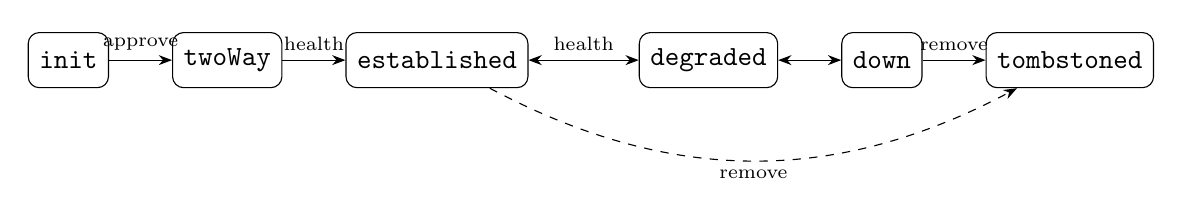
\begin{tikzpicture}[
  >=Stealth,
  state/.style={draw, rounded corners, font=\ttfamily, inner sep=4pt, minimum height=7mm}]
\node[state] (init) {init};
\node[state, right=8mm of init] (two) {twoWay};
\node[state, right=8mm of two] (est) {established};
\node[state, right=14mm of est] (deg) {degraded};
\node[state, right=8mm of deg] (down) {down};
\node[state, right=8mm of down] (tomb) {tombstoned};
\draw[->] (init) -- node[above,font=\scriptsize]{approve} (two);
\draw[->] (two) -- node[above,font=\scriptsize]{health} (est);
\draw[<->] (est) -- node[above,font=\scriptsize]{health} (deg);
\draw[<->] (deg) -- (down);
\draw[->] (down) -- node[above,font=\scriptsize]{remove} (tomb);
\draw[->,dashed] (est) to[bend right=28] node[below,font=\scriptsize]{remove} (tomb);
\end{tikzpicture}}
\caption{OGP federation lifecycle (OSPF-inspired). Human approval advances
\texttt{init}$\to$\texttt{twoWay}; the first bidirectional health check
reaches \texttt{established}. Health changes oscillate through
\texttt{degraded}/\texttt{down}; either party's removal tombstones the peer,
and re-federation requires fresh human approval---there is no silent return
to trust.}
\label{fig:lifecycle}
\end{figure}

\subsection{Three-Layer Scope Model}

OGP enforces scope at three distinct layers, preventing any single
bypass from exposing the full capability surface:

\begin{description}
\item[Layer 1 --- Capability Advertisement] The gateway publishes what
  it \emph{can} support in its discovery card. Peers cannot request
  capabilities not in this list.
\item[Layer 2 --- Per-Peer Grant] At approval time, the approving human
  sets exactly what this specific peer \emph{will} be granted:
  a set of intents, optional topic restrictions for \texttt{agent-comms},
  and a per-intent sliding-window rate limit (e.g., 100 requests/3600 s).
  Grants can be updated at any time without re-federation.
\item[Layer 3 --- Runtime Enforcement (Doorman)] The Doorman validates
  every incoming message against the peer's current grant.
  It checks peer identity, approval status, intent coverage, topic
  allowlist, and rate limit in sequence before any message reaches
  the local agent.
\end{description}

The separation between Layer 2 (stored grant) and Layer 3 (runtime
evaluation) means grants can be tightened mid-relationship without
protocol overhead: the Doorman re-reads the stored grant on each request.

\subsection{Agent-to-Agent Communication (Agent-Comms)}

Beyond raw message passing, OGP includes a structured
\texttt{agent-comms} intent for natural-language agent-to-agent
dialogue. Messages carry a \emph{topic} (e.g., \texttt{project-updates},
\texttt{signal}) that is independently scoped in the peer's grant.

The receiving gateway applies a 7-layer policy precedence chain to
determine how the local agent should handle the message---from a global
default down to a peer-and-topic-specific override:

\begin{enumerate}
\item Legacy inbound policy mode (safety fallback)
\item Global default response level
\item Peer-specific default
\item Global message-class rule (\texttt{human-relay}, \texttt{agent-work}, etc.)
\item Peer message-class override
\item Global topic-level rule
\item Peer topic-level override
\end{enumerate}

Response levels range from \texttt{full} (share everything) through
\texttt{summary}, \texttt{escalate} (ask the human first), and \texttt{off}
(signed rejection with reason---not a silent drop).

\subsection{Signed Project Contributions}

For cross-organizational project coordination, OGP provides a signed
contribution system. When a gateway logs a contribution, the CLI:

\begin{enumerate}
\item Mints a sortable ULID as the stable cross-federation ID
\item Constructs a canonical record:
  \texttt{\{id, projectId, authorId, entryType, summary, timestamp\}}
\item Signs the canonical JSON with the gateway's Ed25519 private key
\item Stores the signed envelope locally and pushes it to peer gateways
\end{enumerate}

\texttt{authorId} is the gateway's Ed25519 public key---no separate key
distribution is needed. On receipt, the Doorman verifies: (1) the signature
is valid, (2) the signed \texttt{authorId} matches the federation-authenticated
sender, and (3) the signed \texttt{projectId} matches the target project.
Any mismatch is a \texttt{401}. A contribution carries one stable ULID
across every gateway it is pushed to.

\subsection{Transport Independence}
\label{sec:transport}

OGP separates the protocol from the transport. The current reference
implementation supports three modes:

\begin{description}
\item[Direct] Peers reach each other via their configured \texttt{gatewayUrl}
  (permanent Cloudflare tunnel, ngrok, VPS, or cloud endpoint).
\item[Relay] Messages route through the optional Rendezvous relay for
  gateways that cannot receive inbound connections directly.
\item[Future] The protocol carries a signed transport descriptor in
  the discovery card, enabling future transports (e.g., Iroh P2P) without
  protocol changes.
\end{description}

%%------------------------------------------------------------------
\section{Security Analysis}
%%------------------------------------------------------------------

\subsection{Threat Model}

OGP's threat model: two gateways, owned by different humans who do not
necessarily trust each other's organizations, each running an AI agent
framework behind a TLS endpoint. The adversary can intercept, replay,
or forge messages; can attempt to establish unauthorized federation;
or can attempt to exceed granted scope.

\subsection{Cryptographic Guarantees}

All messages carry an Ed25519 signature over the canonical JSON
serialization of the payload, including a freshness timestamp.
Verification at the Doorman provides:
\begin{itemize}
\item \textbf{Authenticity}: the message was produced by the holder of
  the sender's private key.
\item \textbf{Integrity}: the payload has not been modified in transit.
\item \textbf{Replay resistance}: the 5-minute timestamp window and
  per-message nonces prevent replayed messages from being accepted.
\item \textbf{Non-repudiation}: each contribution carries its author's
  public key in the signed bytes, making forgery detectable.
\end{itemize}

Key generation uses Node.js's \texttt{node:crypto} Ed25519 implementation.
On macOS, private keys are stored in an instance-specific Keychain entry
derived from the state directory path; on non-macOS, private keys are
encrypted at rest using an operator-provided secret.

\subsection{Authorization Guarantees}

The three-layer scope model means that a compromised peer cannot exceed
its granted permissions even if it can generate valid signatures:
the Doorman enforces the grant independently of the message content.
A peer granted \texttt{agent-comms} on topics \texttt{general} and
\texttt{project-updates} cannot invoke \texttt{project.contribute}
or send an \texttt{agent-comms} message on topic \texttt{finance}---
both are rejected at Layer 3 before the message reaches the local agent.

\subsection{Limitations}

OGP does not address:
(1)~compromise of the gateway host itself (key exfiltration, process
injection)---this is outside the protocol's scope;
(2)~prompt injection in message content that manipulates the receiving
agent's behavior after delivery---this requires defenses at the agent layer;
(3)~denial-of-service against the Rendezvous service (which is optional;
its failure is graceful).

%%------------------------------------------------------------------
\section{Implementation and Evaluation}
%%------------------------------------------------------------------

\subsection{Reference Implementation}

OGP is implemented as a Node.js daemon (\texttt{@dp-pcs/ogp}, MIT license,
v0.11.3 as of this writing)~\cite{ogp2025}. The daemon runs alongside any AI
framework on a separate port and communicates with the local agent via
\texttt{POST /hooks/agent}.
The core daemon comprises approximately 20{,}000 lines of TypeScript
(\texttt{src/}), with additional code in the companion app, rendezvous
server, and menu-bar monitor, across nearly 400 commits spanning three
months of active development.

Key implementation components:
\begin{description}
\item[\texttt{src/shared/signing.ts}] Ed25519 sign/verify using Node.js
  built-in \texttt{node:crypto}. \texttt{signCanonical()} adds a
  freshness timestamp and returns the exact JSON bytes alongside the
  signature so verifiers operate on the same bytes that were signed.
\item[\texttt{src/daemon/doorman.ts}] Three-layer runtime enforcement.
  Checks peer status, finds the applicable scope grant via
  \texttt{findScopeGrant()}, evaluates topic coverage, and enforces
  a sliding-window rate limit using an in-memory timestamp store.
\item[\texttt{src/daemon/peers.ts}] Peer storage with the full federation
  lifecycle state machine (\texttt{deriveFederationState()}).
\item[\texttt{src/daemon/contribution-signing.ts}] Per-contribution
  ULID generation, canonical serialization, and Ed25519 signing.
\end{description}

The implementation includes a reference Rendezvous server
(\texttt{packages/rendezvous}), a macOS companion desktop app
(\texttt{ogp-companion}, Tauri/React), a macOS menu bar monitor, a
marketing website (\texttt{ogp.elelem.expert}), and four Claude Code
skills (\texttt{ogp}, \texttt{ogp-agent-comms}, \texttt{ogp-project},
\texttt{ogp-expose}).

\subsection{Microbenchmarks}

We measured the overhead of OGP's cryptographic and enforcement layers
on Apple M4 Pro (Node.js v26.3.0).
All measurements use \texttt{performance.now()} with batch timing to
achieve sub-microsecond resolution.

\begin{table}[h]
\centering
\caption{OGP microbenchmark results (Apple M4 Pro, Node.js v26.3.0, n$\geq$5{,}000).}
\label{tab:bench}
\small
\begin{tabular}{lrrl}
\toprule
Operation & Mean & p99 & Notes \\
\midrule
Ed25519 sign & 19\,$\mu$s & 31\,$\mu$s & 52{,}632 ops/sec \\
Ed25519 verify & 44\,$\mu$s & 69\,$\mu$s & 22{,}573 ops/sec \\
HMAC-SHA256 sign & 8\,$\mu$s & --- & 2.3$\times$ faster (weaker identity) \\
Full msg lifecycle & 65\,$\mu$s & 95\,$\mu$s & sign + verify + timestamp \\
Signed contribution & 86\,$\mu$s & 135\,$\mu$s & ULID + sign + verify \\
3-layer scope eval & $<$1\,$\mu$s & 1.2\,$\mu$s & capability+grant+rate-limit \\
7-layer policy chain & $<$1\,$\mu$s & $<$1\,$\mu$s & all precedence layers \\
Doorman (1 peer) & 0.1\,$\mu$s & 0.7\,$\mu$s & Map lookup + grant find \\
Doorman (1000 peers) & $<$1\,$\mu$s & $<$1\,$\mu$s & hash map; no linear scan \\
\bottomrule
\end{tabular}
\end{table}

The Ed25519 sign/verify cycle (19\,$\mu$s / 44\,$\mu$s) dominates the
per-message overhead, as expected for an asymmetric signature scheme.
The 2.3$\times$ overhead versus HMAC-SHA256 is the cost of non-repudiable
per-message authorship: HMAC provides only shared-secret integrity, not
individual identity. The Doorman and policy-resolution layers add
sub-microsecond overhead independent of federation scale---the Map-based
peer store does not degrade with peer count.

In aggregate, an OGP gateway adds approximately 65\,$\mu$s per message
for the sign+verify+authorization path. For agent-to-agent communication,
where message round-trips are measured in seconds (agent reasoning time),
this overhead is negligible.

\subsection{Deployment Case Study}

OGP has been running across several independent gateways on distinct
infrastructure and in different geographic locations
(Table~\ref{tab:deploy}). Each federation was established by explicit
human approval on both sides, then operated autonomously under per-peer
scope and response-level policy.

\begin{table}[h]
\centering
\caption{Active OGP federations: independent operators, infrastructure, and transports.}
\label{tab:deploy}
\small
\begin{tabular}{p{0.20\columnwidth}p{0.30\columnwidth}p{0.16\columnwidth}p{0.20\columnwidth}}
\toprule
Peer & Infrastructure / location & Transport & Autonomy \\
\midrule
Cosmo (AI CoE agent) & OpenClaw on AWS (``Clawporate''), always-on & Direct (Cosmo-advertised) & Full (no human in loop) \\
Stephen Barr & Self-hosted, Seattle, USA & Direct (tunnel) & Escalate / summarize \\
Stanislav Huseletov & Self-hosted, Spain & Direct (tunnel) & Escalate-on-need \\
\bottomrule
\end{tabular}
\end{table}

\noindent\textbf{Mixed transports interoperate.} Transport choice is
per-gateway and advertised in the discovery card; peers need not agree.
The author's gateway advertises \texttt{relay} (so inbound peers reach it
through the Rendezvous relay, removing the need to run a tunnel), while
Cosmo advertises \texttt{direct} (so the author's gateway reaches Cosmo's
AWS endpoint directly). A single federation thus spans two transport modes
without protocol change---validating the transport-independence design of
\S\ref{sec:transport} in production.

\vspace{0.3em}
\noindent\textbf{Autonomous agent-to-agent operation (Cosmo).}
Cosmo is the Center of Excellence's standing agent: it ingests structured
updates from member organizations and answers user queries so that humans
do not have to. CoE leaders' gateways push updates to Cosmo over the
\texttt{project.contribute} intent and converse over \texttt{agent-comms};
Cosmo aggregates this state and republishes it to an external website.
This is delivered as an \emph{OGP App} (``Signal''): a declarative
manifest that advertises the project intents it consumes and installs
the skills CoE leaders use to drive their own agents. The entire pipeline
runs with \emph{no human in the loop} by design---Cosmo's inbound policy
is set to \texttt{full} for the granted topics. Critically, this does not
weaken the trust model: a human approved the federation once, fixing the
scope; the Doorman then enforces that scope on every message
autonomously. Cosmo can receive project updates and answer queries on
approved topics, but cannot invoke any intent or topic outside its
grant---the access decision never reaches Cosmo's underlying agent.

\vspace{0.3em}
\noindent\textbf{Human-mediated collaboration (Stephen, Stanislav).}
The federation with Stephen Barr (Seattle) has run for roughly a month
over a direct tunnel. The federation with Stanislav Huseletov (Spain) has
run since the second week of the project; the two gateways coordinated
real design and test work---iterating on a candidate website via
\texttt{project} intents and \texttt{agent-comms}, with the agents
handling routine exchange and escalating to their humans only when a
decision was required. These links exercise the \texttt{escalate} and
\texttt{summarize} response levels, in contrast to Cosmo's fully
autonomous \texttt{full} level---demonstrating that the same protocol
spans the full autonomy spectrum under per-peer human-set policy.

\vspace{0.3em}
All federations have survived gateway restarts, tunnel URL rotations,
transport switches, and software upgrades without re-federation---the
public key is the durable identity, not the gateway URL or transport.

%%------------------------------------------------------------------
\section{Discussion}
%%------------------------------------------------------------------

\subsection{What OGP Does Not Solve}

OGP solves trust establishment and scope enforcement at the gateway
boundary. It does not solve:

\begin{description}
\item[NAT traversal] OGP requires each gateway to be publicly reachable.
  The relay transport provides a workaround for gateways behind strict NAT,
  but peer-to-peer hole punching is out of scope for this protocol version.
\item[Message content semantics] OGP delivers authenticated, scoped messages.
  What the receiving agent does with them---and whether it can be
  manipulated by prompt injection within the message content---is a
  matter for the agent layer, not the gateway layer.
\item[Group federation] OGP is strictly point-to-point.
  Multi-party federation (three or more gateways in a mesh) requires
  pairwise peering; OGP does not define a group membership protocol.
\item[Revocation propagation] When a gateway is compromised,
  its peers must be individually notified. There is no broadcast
  revocation mechanism.
\item[Human-factors of approval] OGP's central premise---that a human is
  the right arbiter of federation---is a design position, not yet an
  empirical result. Whether operators set scopes correctly and understand
  what they grant is the key open question, and the subject of ongoing work.
\end{description}

\subsection{OGP Apps: A Distribution Layer}

A natural extension of trusted gateway relationships is software
distribution through them. OGP Apps (\texttt{ogp-app.json} manifests)
let peers advertise declarative capability bundles---specifying which
intents they fire, which skills they install into the recipient's AI
agent, and where their output lives. Installation goes through a
consent gate (the human sees exactly which scripts run and which
intents are used before confirming). The federation trust relationship
doubles as a software distribution channel, scoped to the same
bilateral approval model.

\subsection{Relationship to Emerging Standards}

OGP is not a competing standard---it is a complement to the emerging
agent protocol ecosystem. We anticipate that OGP gateways will use
A2A for intra-org task delegation, MCP for tool attachment, and ANP
for public web discovery, while OGP governs what crosses the
organizational boundary. The gateway is the right abstraction for this
role: a durable, human-controlled trust boundary that outlasts any
individual agent session.

The cleanest framing: A2A is HTTP, enabling request/response between
services. OGP is BGP, establishing the policy framework between autonomous
systems before any requests flow.

%%------------------------------------------------------------------
\section{Conclusion}
%%------------------------------------------------------------------

We presented OGP, a federation protocol that applies BGP's peering
model to AI gateway interoperability. OGP's defining properties---mandatory
human approval for federation establishment, three-layer scope enforcement,
Ed25519 per-message authentication, and unilateral revocability with
cryptographic tombstoning---address a gap that no existing agent protocol
fills. The reference implementation demonstrates sub-millisecond enforcement
overhead at every layer, confirming that the security model does not impose
meaningful latency costs on agent communication. Active deployment between
two organizational gateways validates the protocol under real cross-boundary
collaboration conditions.

The protocol specification, reference implementation, and benchmarks are
available at \url{https://github.com/dp-pcs/ogp}.

%%------------------------------------------------------------------
\bibliographystyle{ACM-Reference-Format}
\bibliography{hotnets2026}

\end{document}
